86. Сначала посчитаем, сколько клеток в исходном прямоугольнике: их 37. После это надо приложить букву $L$ всеми возможными способами и посмотреть, сколько клеток она может добавить. При этом надо не забывать, что фигуру можно как поворачивать, так и переворачивать.
\begin{figure}[ht!]
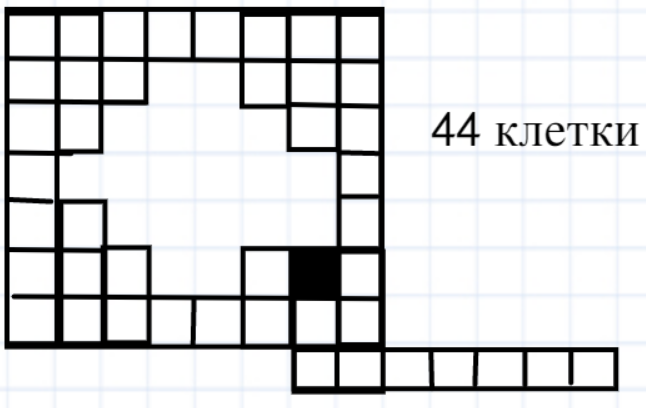
\includegraphics[scale=0.35]{l1.png} 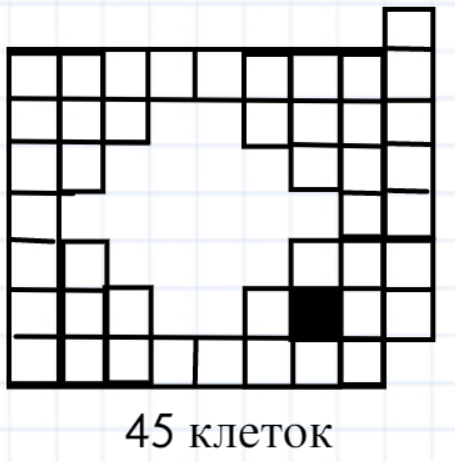
\includegraphics[scale=0.35]{l2.png}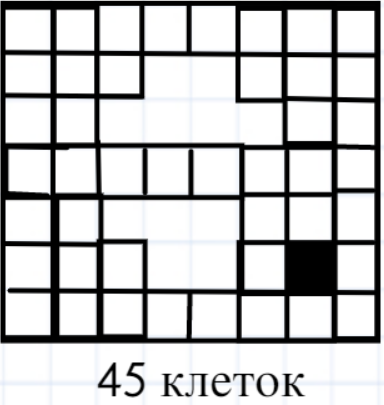
\includegraphics[scale=0.35]{l3.png}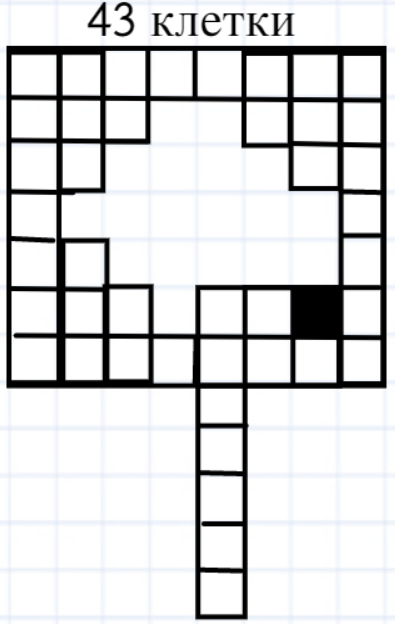
\includegraphics[scale=0.35]{l4.png}\end{figure}
\begin{figure}[ht!]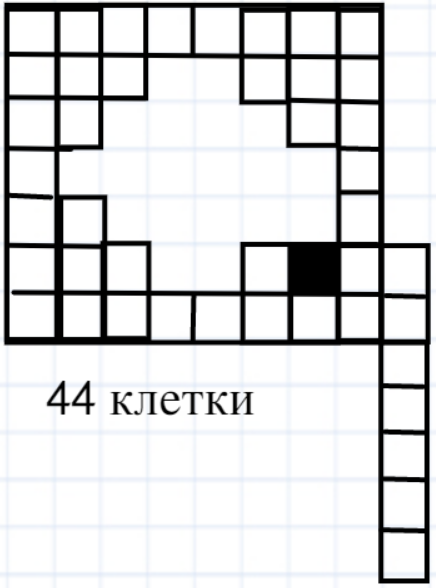
\includegraphics[scale=0.35]{l5.png} 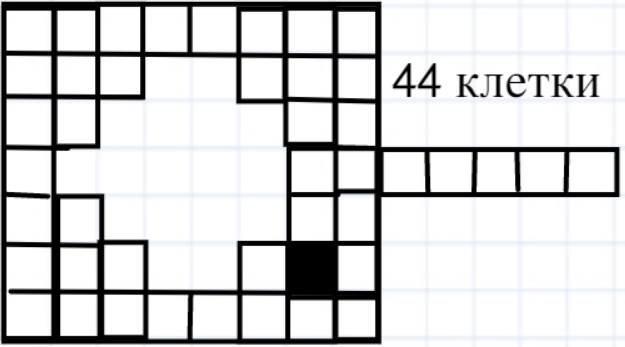
\includegraphics[scale=0.35]{l6.png}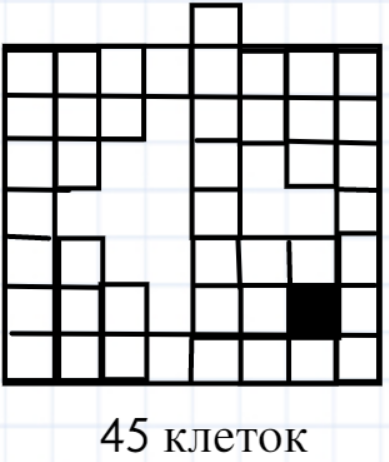
\includegraphics[scale=0.35]{l7.png}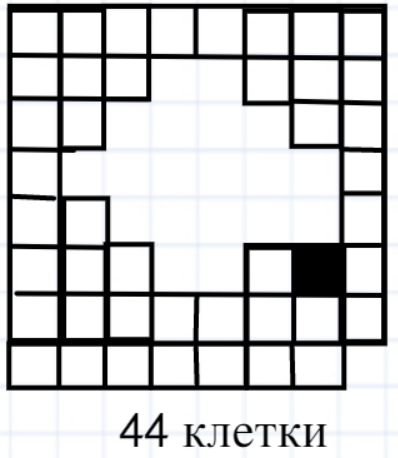
\includegraphics[scale=0.35]{l8.png}
\end{figure}\\
Как мы видим, возможны всего три варианта: 43, 44 или 45 клеток.

ewpage
oindent
